% This is samplepaper.tex, a sample chapter demonstrating the
% LLNCS macro package for Springer Computer Science proceedings;
% Version 2.21 of 2022/01/12
%
\documentclass[runningheads]{llncs}
%
\usepackage[T1]{fontenc}
% T1 fonts will be used to generate the final print and online PDFs,
% so please use T1 fonts in your manuscript whenever possible.
% Other font encondings may result in incorrect characters.
%
\usepackage{graphicx}
% Used for displaying a sample figure. If possible, figure files should
% be included in EPS format.
%
% If you use the hyperref package, please uncomment the following two lines
% to display URLs in blue roman font according to Springer's eBook style:
%\usepackage{color}
%\renewcommand\UrlFont{\color{blue}\rmfamily}
%\urlstyle{rm}
%

% ==================== my packages ====================
\newcommand{\printnombrecomision}{Comisión Especial de Estadística de
  Seguridad, Justicia, Crimen y Transparencia}
\newcommand{\printInicialesComision}{CEESJCT}
\newcommand{\modelohuggingface}{distilbert-base-multilingual-cased}
\usepackage{numprint}
\usepackage{dirtytalk}
\usepackage{amsmath, bm}
\usepackage{amssymb}
\usepackage{amsfonts}
\usepackage{mathrsfs}
\usepackage{mathtools}
\usepackage{csquotes}
\usepackage{tabularx}
\usepackage{multirow}
\usepackage{booktabs}
\DeclareMathOperator{\ypred}{\phi}  %options \hslash
\DeclareMathOperator{\ypredtarget}{\phi^{T}}
\DeclareMathOperator{\ypredsource}{\phi^{S}}
\DeclareMathOperator{\ConvNetOut}{\mathcal{A}}
\DeclareMathOperator{\Tokenization}{\Gamma}
\DeclareMathOperator{\Tokenize}{Tokenize}

\newcommand{\bertmodel}{\textsc{BERT}}

% ==================== prompt ====================

% You are computer science PhD professional. Your task is to assist me
% to improve the writing of scientific articles. This may involve
% summarize and re-phrase. The article is written in Latex so mastery in
% the use of Latex is expected.

\begin{document}
%
\title{BERT-Based Fine-Tuning for Automated Tagging of Robbery Crime  Narratives}

%
\titlerunning{Fine-Tuning BERT for Robbery Narrative Tagging}
% If the paper title is too long for the running head, you can set
% an abbreviated paper title here
%
\author{Lenin G. Falconi\inst{1}\orcidID{0000-0003-4402-6643} \and\\
Myriam Hernandez-Alvarez\inst{1}\orcidID{0000-0003-4718-0400} \and\\
Ángel Leonardo Valdivieso Caraguay\inst{1}\orcidID{0000-0002-3502-020X}}
%
\authorrunning{L. Falconi et al.}
% \authorrunning{Lenin G. Falconi \and Myriam Hernandez-Alvarez \and
%   Leonardo Valdivieso}
% First names are abbreviated in the running head.
% If there are more than two authors, 'et al.' is used.
%
% \institute{Princeton University, Princeton NJ 08544, USA \and
% Springer Heidelberg, Tiergartenstr. 17, 69121 Heidelberg, Germany
% \email{lncs@springer.com}\\
% \url{http://www.springer.com/gp/computer-science/lncs} \and
% ABC Institute, Rupert-Karls-University Heidelberg, Heidelberg, Germany\\
% \email{\{abc,lncs\}@uni-heidelberg.de}}

\institute{Escuela Politécnica Nacional, Quito 170525, Ecuador\\
\url{https://www.epn.edu.ec} \\
\email{\{lenin.falconi,myriam.hernandez,angel.valdivieso\}@epn.edu.ec}}
%
\maketitle              % typeset the header of the contribution
%
% abstract 150 -- 250 words
\begin{abstract}
  Accurate classification of crime narratives is vital for reliable
  public safety statistics. In Ecuador, Comisión Especial de
  Estadística de Seguridad, Justicia, Crimen y Transparencia (CEESJCT)
  manually categorizes robbery incident reports, which is a
  time-consuming process. While transformer-based models have shown
  success in natural language processing tasks, their application to
  Ecuadorian legal and security texts in the Spanish language,
  underexplored. This study addresses this gap by developing an
  automated classification system using a BERT model tailored to
  Spanish robbery narratives. Utilizing transfer learning and
  subsequent fine-tuning on an expanded, labeled dataset, the system
  significantly improved classification performance. Initial transfer
  learning achieved moderate accuracy (80.5\%) but faced difficulties
  with semantically similar categories. Fine-tuning notably increased
  minority-class recall (up to 30\%) with an improved accuracy
  (90.3\%). The final implementation, which increased the number of
  categories to 11, achieved 95.5\% accuracy with robust and
  consistent results on both police and judicial narratives. 
  Collaboration with Ecuadorian institutions, including the Fiscalía
  General del Estado (FGE) and Instituto Nacional de Estadística y
  Censos (INEC), ensured model credibility.
  
  \keywords{Legal Natural Language Processing \and NLP \and Natural
    Language Processing \and transformers \and fine-tuning \and
    transfer learning.}
\end{abstract}
%
%
%

\section{Introduction}
Deep learning models (DL) have yielded remarkably
successful outcomes across a wide range of applications (e.g., image
classification, object detection, natural language
processing)\cite{PATHAK20181706}. In various text classification
tasks, such as sentiment analysis, news categorization,
question-answering, and natural language inference, DL has outperformed
traditional \emph{Machine Learning (ML)}  methods\cite{Minaee2021}, a
testament primarily to its inherent generalization and
robustness\cite{Zahangir2018}. However, depending on the problem
to be solved, designing a DL architecture demands a substantial volume
of data to attain the desired generalization performance. For example,
in image processing and computer vision, datasets such as ImageNet
(\numprint{14197122}) and Microsoft COCO (\numprint{2.5} million)
provide extensive data per category\cite{PATHAK20181706}, while in
\emph{Natural Language Processing (NLP)}, resources like WebTex, composed of
millions of web pages, have been pivotal in training models such as
GPT-2\cite{radford2019language}.

Although the success of DL hinges on large datasets, specialized
hardware \cite{radford2019language}\cite{murphy2022probabilistic}, and
model architecture, for niche domains with limited data,
\emph{Transfer Learning (TL)} and \emph{Fine-Tuning (FT)} enable
knowledge transfer from source to target domains by reusing
early-layer features and adapting task-specific layers
\cite{yosinski2014transferable}\cite{howard2018universallanguagemodelfinetuning}.The
legal documentation domain is a promising field for applying NLP,
where digital information can be leveraged to develop tools that
optimize legal workflows. However, applications face language
limitations, as LexGlue, the most widely used benchmark, focuses on
English despite the growing interest in judicial outcomes
prediction\cite{mumcuouglu2021natural,kalia2022classifying,wang2020deep},
legal article prediction from text and document classification
\cite{yan2019law,clavie2021}. While transformers models like mBERT
enable cross-lingual transfer, legal terminologies and system
differences necessitate domain-specific
pretraining (e.g., LegalBERT \cite{chalkidis2020legal}) or hybrid
approaches \cite{liu2022legal}, particularly for low-resource
languages \cite{savelka2021cross}.

In Ecuador’s penal code (COIP), robbery is defined in Article
189. However, subclassifications such as home robbery\footnote{robo a
  domicilio}, street robbery\footnote{robo a personas}, robbery of
businesses\footnote{robo a unidades económicas}, vehicle part
theft\footnote{robo de bienes, accesorios y autopartes de vehículos},
car theft\footnote{robo de automóviles}, and motorcycle
theft\footnote{robo de motocicletas} are used primarily for public
security analytics and manually identified by the
\textit{\printnombrecomision}\ (CEESJCT) using \textit{crime incident
  reports}\footnote{Noticia del Delito}. To automate this, we propose
a transformer-based classifier that uses multilingual DistilBERT
\cite{Sanh2019DistilBERTAD}.  We implemented a three-phase approach:
\textbf{Phase 1: Classification with transfer learning} the
transformer model is used as a feature extractor followed of full
connecting layers and dropout achieving 80.5\% accuracy (F1:
0.80). Even though the model’s bidirectional attention mechanism and
subword tokenization (WordPiece) proved essential for capturing
semantic relationships in crime narratives, particularly when some
words remain misspelled and uncorrected for legal reasons protecting
the victim's statement, it struggled with minority
classes. \textbf{Phase 2: Fine-Tuning for Contextual Adaptation} Using
a learning rate $5 \times 10^{-5}$) improved accuracy to 90.3\% (F1:
0.90) by resolving semantic ambiguities and achieving significant
gains for less frequent categories. Additionally, a Flask web
application was deployed for real-time predictions, which demonstrated
an accuracy of 89\% on unseen CEESJCT data. Stages 1 and 2 used a
dataset of 431,669 robbery reports (2014–2022), tokenized into
sequences of up to 300 words, and split into training (63\%),
validation (16\%), and test (21\%) sets. \textbf{Phase 3: Scaling to
  Complex Taxonomies} model is fine tuned to predict a total of 11
categories, extending the original 6. A merged validated dataset of
1.1 million narratives was developed by combining police reports with
criminal complaints filed in the prosecutor's office. The model was
trained using TPU to process the entire dataset. A notable improvement
in accuracy performance was achieved (95.5\% accuracy with an F1-score
of 0.95).

% Notably, the baseline TL model achieved moderate accuracy (80.5\%) but
% struggled with semantically overlapping categories. FT resolved many
% of these issues, improving minority-class recall by up to 30\%. The
% final scaled model demonstrated high robustness (95.5\% accuracy) on
% 11 categories. Challenges persisted for low-frequency classes with
% limited training samples. However, it could suggest new grouping rules
% for the commission to consider. What is more, Semantic similarity
% analysis revealed near-identical embeddings (98.7\% cosine similarity)
% between police and prosecutor's reports, validating the model’s
% consistency across different data sources.

The structure of this article is organized as follows. Section
\ref{chap:literatura} provides a comprehensive literature review on
text classification challenges, along with theoretical foundations of
\emph{Transformers}, TL and FT. Section
\ref{sec:methods} describes the methodology developed for dataset
construction and model training. Experimental results are presented in
Section \ref{chap:resultados}. Finally, Section \ref{chap:conclusion}
discusses the findings while Section \ref{chap:futuro} outlines future
research directions.

\section{Foundational Concepts and Related Works}\label{chap:literatura}
In this research, we propose a transformer-based model for robbery
offense classification aligned with categorical frameworks established
by both the Prosecutor's Office and INEC.  Legal documents present
unique challenges compared to general-domain texts, characterized by
three distinctive features: (1) inherent structural complexity, (2)
substantial document length, and (3) specialized juridical
terminology. These characteristics have led to the emergence of Legal
Natural Language Processing (LNLP) as a specialized NLP subdomain
\cite{Ariai2024,Zhong2020}.

Within this paradigm, Legal Text Classification (LTC) refers to the
task of categorizing legal documents into predefined juridical
categories. While LTC shares fundamental principles with general TC,
it introduces specific technical challenges including but not limited
to: high class cardinality (typically ranging from dozens to hundreds
of categories), multi-label classification requirements, and the need
for domain-specific feature engineering. The complexity of LTC
increases exponentially with the number of potential legal categories
and their hierarchical relationships within juridical systems.


% Transformer-based models have demonstrated significant improvement in
% TC, primarily due to their ability to capture long-range dependencies
% and contextual relationships within the text
% \cite{Allam2025}\cite{vaswani2017attention}, demonstrating an ability
% to understand subtle nuances withing a language. This capability is
% important when dealing with the intricate nature of legal texts
% \cite{Ariai2024}.

% The inherent complexity, substantial length, and specialized
% terminology characteristic of legal texts present significant
% challenges for manual processing and analysis
% \cite{Ariai2024}.  Hence AI models in legal applications must follow
% strict standards for accuracy to mitigate bias, unfairness and
% explainability issues \cite{Ariai2024}. Therefore, \textit{Legal
%   Artificial Intelligence (LAI)} specializes in the application of AI
% in the legal domain \cite{Zhong2020}. Some of the important research
% areas are: \textit{Legal Argument Mining (LAM)}, \textit{Legal Text
%   Classification (LTC)}, \textit{Legal Named Entity Recognition
%   (LNER)}, \textit{Legal Document Summarization (LDS)}, \textit{Legal
%   Judgement Prediction (LJP)}, \textit{Legal Question Answering (LQA)}

% \subsection{Background Concepts}
% \label{sec:background-concepts}


\subsection{Legal Natural Language Processing}
\label{sec:legal-lang-proc}
% Legal Natural Language Processing (LNLP)represents the application of
% NLP techniques, architectures, and models to legal documents
% \cite{Ariai2024}\cite{Zhong2020}. In many contexts, however, the terms
% LNLP and legal AI (LAI) are used interchangeably, as both refer to
% employing advanced computational methods in the legal
% domain. According to \cite{Ariai2024}, legal documents are
% characterized by their precise use of formal vocabulary and complex
% syntax to minimize ambiguity, frequent employment of specialized,
% often archaic, terminology, extensive intertextuality through
% references to other legal texts, and considerable document length,
% which collectively present significant challenges for processing and
% interpretation.

NLP for legal documents primarily focus on two categories
of approaches: \textit{Embedding Methods} and \textit{Symbol-Based
  Methods} \cite{Zhong2020}. Embedding Methods, such as
transformer-based models (e.g., BERT), derive high-level
representations from large corpora and offer strong predictive
performance, but their opacity raises concerns about
interpretability. Conversely, Symbol-Based Methods explicitly model
legal knowledge and facilitate reasoning over structured
representations, thereby providing greater transparency, though often
at the expense of accuracy. Recent work in explainable AI seeks to
address this limitation in embedding methods.For example,
attention-based techniques such as \textit{attention rollout} and
\textit{attention flow} aggregate attention weights across layers in
transformers, offering insight into model decisions and revealing a
degree of inherent explainability \cite{Abnar2020}.

The Transformer architecture, introduced in
\cite{vaswani2017attention}, represents a significant advancement in
NLP by incorporating a self-attention
mechanism that allows deep learning models to effectively capture
long-range dependencies and facilitates efficient parallel
training. This innovation supplanted the previous state-of-the-art
recurrent neural network (RNN) approaches, including Long Short-Term
Memory (LSTM) networks \cite{tunstall2022natural}. Transformers employ
an encoder-decoder architecture augmented by self-attention and
transfer learning (TL) methodologies.

BERT \cite{devlin2018bert}, a notable application of the Transformer
encoder, generates deeply bidirectional contextual representations
through exclusively encoder-based architecture. Its pre-training
utilizes self-supervised objectives such as masked language modeling
(MLM) and next sentence prediction (NSP), enabling the model to
acquire rich contextual information from extensive corpora.

% \subsubsection{Legal Text Classification (LTC)}
% \label{sec:legal-text-class}
% \subsection{Foundational Concepts and Background}
% \subsubsection{Text Classification}
% \subsubsection{Legal Text Classification}
% \subsubsection{NLP versus Legal NLP}
% \subsubsection{Transformer Models in NLP and LTC}
% Common methods use: SVM, CNN and \textit{Recurrent Neural
%   Networks(RNN)}. Most advanced methods use transformer-based models
% like Legal-BERT \cite{chalkidis2020legal}, RoBERTa where the models
% are essentially fine-tuned on annotated legal datasets to handle a
% large number of possible legal categories \cite{Ariai2024}. In this
% research, the problem faced corresponds to multi-class classification
% with at most 11 categories.

% \subsubsection{The Transformer Architecture}
% \label{sec:transf-architecture}


% A key strength of BERT lies in its use of the WordPiece tokenization
% algorithm, which decomposes words into subword units, thereby
% addressing the Out of Vocabulary (OOV) problem by allowing unfamiliar
% words to be represented through more frequent root, prefix, and suffix
% components. This property is particularly beneficial in specialized
% domains like law, where domain-specific adaptations—such as
% Legal‑BERT—have been developed. Legal‑BERT extends BERT’s architecture
% and is further pre-trained on legal corpora to better capture the
% specialized terminology, syntax, and reasoning characteristic of legal
% texts \cite{chalkidis2020legal}.

\subsection{Related Works}
\label{sec:related-works}
% In this research, we present a model for theft classification
% according to statistical categories defined by the prosecutor's office
% as well as the INEC. By examining the methodologies, datasets, and
% findings of these related works, we try to assess the potential
% uniqueness of our current work. In Table \ref{tab:work-summary}.
This section reviews related work in LTC research, focusing on three
critical dimensions: (1) architectural innovations, (2) dataset
characteristics and domain adaptation strategies, and (3) comparative
performance. Table \ref{tab:work-summary} provides a  comparison of these
approaches. While existing research has predominantly focused on
English-language legal corpora our work represents, to our knowledge,
innovative in exploring transformer architectures in Spanish legal
documents attached to Ecuadorian reality.

In their research work, \cite{Shaheen2020} tackle large-scale
multi-label legal text classification using transformer architectures
(BERT, RoBERTa, DistilBERT, XLNet, M-BERT). Through systematic
evaluation on the JRC-Acquis (multilingual) and EURLEX57K (English)
datasets, they demonstrate that combining gradual layer unfreezing,
discriminative learning rates, and domain-specific pretraining
achieves state-of-the-art performance; surpassing LSTM baselines by
significant margins. The authors further propose standardized dataset
splits to facilitate reproducible research, establishing transformers
as the new benchmark for legal document classification with complex
taxonomies like EuroVoc.

\cite{Shaheen2021} extends this research to zero-shot cross-lingual
transfer using multilingual transformers (M-BERT, M-DistilBERT). By
fine-tuning models exclusively on English EURLEX57K documents and
evaluating on French/German translations, they achieve target-language
performance comparable to models trained on all three languages. Key
innovations include continued pretraining on legal corpora and
progressive unfreezing during fine-tuning, highlighting transformers'
ability to bridge linguistic gaps in low-resource legal NLP scenarios.

The cross-linguistic applicability of transformers is further
validated by \cite{Akca2022} for the classification of Turkish legal
texts. Their comparative analysis reveals that transformer-based
models outperform traditional ML methods (e.g., SVM, logistic
regression) in accuracy, despite limited training
data. While specific classification categories remain unspecified,
this study crucially demonstrates that transformers' superiority
extends beyond English to other languages.

Addressing the challenge of document length, \cite{Vatsal2023}
systematically evaluates BERT adaptations for U.S. Supreme Court
decisions from the Supreme Court Database (SCDB). They find that
domain-adapted Legal-LongFormer and Legal-BERT outperform their
general-domain counterparts. This underscores the significance of
domain-specific pretraining and optimized strategies for handling
lengthy documents in legal text classification. ~\cite{Shaheen2020}

% In \cite{Shaheen2020}, the authors address the complex problem of
% large-scale multi-label text classification in the legal domain,
% focusing on assigning one or multiple labels from the comprehensive
% EuroVoc taxonomy to legal documents. They evaluate several advanced
% transformer models, including BERT, RoBERTa, DistilBERT, XLNet, and
% Multilingual BERT (M-BERT), exploring the impact of various training
% regimes such as generative pretraining, gradual unfreezing of model
% layers, and discriminative learning rates. Experiments are conducted
% on two substantial datasets: JRC-Acquis, a multilingual parallel
% corpus, and EURLEX57K, comprising 57,000 English EU legislative
% documents annotated with EuroVoc labels. The study achieves new
% state-of-the-art results on the JRC-Acquis dataset and provides a
% quantitative analysis of individual training strategies' effects on
% model performance. Additionally, standardized dataset splits are
% proposed to support future research. Overall, this work establishes a
% significant benchmark for the use of transformer models in large-scale
% legal text classification, evidencing their superior
% performance—particularly over LSTM architectures—when applied to
% extensive legal documents and complex topic taxonomies.

% Further extending this line of research, \cite{Shaheen2021}
% investigates zero-shot cross-lingual transfer capabilities of
% transformer models for multi-label legal text classification. The
% approach involves training a model on English legal documents with the
% intent of directly applying it to French and German documents without
% target-language training data. Utilizing M-DistilBERT and M-BERT, both
% pretrained on multilingual corpora, the study examines the influence
% of techniques such as language model fine-tuning (i.e., continued
% pretraining on legal corpora) and gradual unfreezing of network
% layers. The EURLEX57K dataset is extended to include French and German
% translations of the English texts. The findings indicate that
% fine-tuning multilingual transformer models on English legal data
% markedly enhances zero-shot performance in French and German, to the
% extent that it is comparable to models trained jointly on all three
% languages. This underscores the potential of multilingual transformer
% models for legal text classification tasks in low-resource languages.

% In \cite{Akca2022}, a comparative analysis of traditional machine
% learning (ML) and deep learning (DL)-based methods, including
% transformer architectures, is conducted for the classification of
% Turkish legal documents. The study evaluates domain adaptation methods
% alongside standard algorithms, considering a dataset of Turkish law
% texts classified into multiple categories. The results demonstrate
% that deep learning models, especially those utilizing transformer
% architectures, consistently surpass traditional ML approaches in
% accuracy. This highlights the efficacy of transformer models for legal
% text classification tasks within a non-English context. However, the
% available information does not detail the specific nature of
% classification categories, nor does it clarify whether crime types
% such as robbery are among them.

% Finally, \cite{Vatsal2023} examines the application of BERT-based
% models for classifying long legal documents, specifically US Supreme
% Court decisions from the Supreme Court Database (SCDB). Given the
% inherent constraint of standard BERT models to process sequences of up
% to 512 tokens, the authors experiment with several strategies for
% accommodating longer texts, such as stride-based chunking (overlapping
% text segments), chunk concatenation, and document summarization. These
% are compared with transformers tailored for long inputs, namely
% LongFormer and Legal-LongFormer (the latter pre-trained on legal
% corpora). The SCDB, annotated with a two-level subject taxonomy (15
% general and 279 fine-grained topics), serves as the evaluation
% benchmark. Results indicate that domain-adapted models (Legal-BERT and
% Legal-LongFormer) generally outperform their general-domain
% counterparts. Among chunking techniques for standard BERT, the
% stride-based approach performs best, while LongFormer variants do not
% surpass chunked BERT models. This underscores the significance of
% domain-specific pretraining and optimized strategies for handling
% lengthy documents in legal text classification. ~\cite{Shaheen2020}

% \begin{table}[htbp]
%     \centering
%     \caption{Comparison of Models and Performance in Literature}
%     \label{tab:work-summary}
%     % Create a table that spans the full text width
%     \begin{tabularx}{\textwidth}{|XXXX|}
%         \hline
%         \textbf{Title} & \textbf{Authors \&  Year} & \textbf{Model} & \textbf{Results} \\
%       \hline
      
%         \citetitle{Shaheen2020} & 
%         \citeauthor{Shaheen2020}, \citeyear{Shaheen2020}  & 
%         BERT, RoBERTa, DistilBERT, XLNet, M-BERT &
%         0.661 (F1) on JRC-Acquis \\
%         % \hline
%         \citetitle{Shaheen2021} &
%         \citeauthor{Shaheen2021}, \citeyear{Shaheen2021} &
%         M-DistilBERT, M-BERT &
%         34\% improvement on French, 87\% improvement on German \\
%       % \hline
%       \citetitle{Vatsal2023} &
%       \citeauthor{Vatsal2023}, \citeyear{Vatsal2023} &
%                                                                                 BERT,
%                                                                                 RoBERTa,
%                                                                                 Legal-BERT,
%                                                                                 LongFormer,
%                                                                                 Legal-LongFormer&
%                                                                                                   80.1\%
%                                                                                                   accuracy
%                                                                                                   (15
%                                                                                                   categories),
%                                                                                                   60.9\%
%                                                                                                   accuracy
%                                                                                                   (279
%                                                                                                   categories)
%                                                                                                   with
%                                                                                                   Legal-BERT\\
%       \citetitle{Akca2022} & \citeauthor{Akca2022},\citeyear{Akca2022}
%                                                    & Transformer-based
%                                                                     &
%                                                                       Deep
%                                                                       learning
%                                                                       models
%                                                                       generally
%                                                                       outperform
%                                                                       traditional
%                                                                       ML\\
%       \hline
      
%     \end{tabularx}
% \end{table}


\begin{table}[ht]
\centering
\caption{Comparative analysis of legal text classification approaches}
\scriptsize
\label{tab:work-summary}
\begin{tabularx}{\textwidth}{p{0.1\textwidth}XXXXp{0.3\textwidth}}
\hline
\textbf{Ref} & \textbf{Model} & \textbf{Task} & \textbf{Dataset} & \textbf{Language} & \textbf{Key Results} \\ 
\hline
\cite{Shaheen2020} & BERT, RoBERTa, DistilBERT, XLNet, M-BERT &
                                                                Multi-label
                                                                classification
                                                                     &
                                                                       JRC-Acquis, EURLEX57K & Multilingual, English  & 0.661 (F1) on JRC-Acquis \\

\cite{Shaheen2021} & M-BERT, M-DistilBERT & Cross-lingual transfer &
                                                                     EURLEX57K
                                                                     Extended
                                                                                        &
                                                                                          Models
                                                                                          pretrained
                                                                                          in
                                                                                          Multilingual. FT
                                                                                          in
                                                                                          English & 34\% improvement on French, 87\% improvement on German \\

\cite{Akca2022} & Transformer-based & Document classification &
                                                                Turkish
                                                                Legal
                                                                Corpus
                                                                                        &
                                                                                          Turkish
                                                                                                            &
                                                                                                              DL
                                                                                                              models
                                                                                                              improve
                                                                                                              over
                                                                                                              traditional
  ML\\

  \cite{Vatsal2023} & BERT, RoBERTa,
                      Legal-BERT,
                      LongFormer,
                      Legal-LongFormer & Long document classification & SCDB & English & 80.1\%
                                                                                         accuracy
                                                                                         (15
                                                                                         categories),
                                                                                         60.9\%
                                                                                         accuracy
                                                                                         (279
                                                                                         categories)
                                                                                         with
                                                                                         Legal-BERT \\
  \hline
\end{tabularx}
\end{table}

\subsection{Discussion, Findings and Contribution}
\label{sec:discussion-findings}
The reviewed literature indicates that BERT models are widely utilized
for legal text classification (LTC). Transformer-based architectures
consistently outperform traditional machine learning methods in this
domain\cite{Akca2022}. Fine-tuning pre-trained BERT weights to the
target task is a standard approach. Also, our methodology is
comparable to that of \cite{Vatsal2023}, wherein models are trained
for both broader and fine-grained legal categories. A recurrent
challenge with BERT-based approaches concerns the processing of
lengthy documents, due to BERT's tokenization limits.

Distinct from previous works, our study specifically addresses the
classification of robbery types. Most literature focuses on broader
legal categories, and while some studies may implicitly include
robbery within categories such as "criminal law" or "property
offenses," explicit attention to robbery classification is absent,
marking our focus as potentially novel and expands the exploration in
application of transformer-based models in legal domain.

Another important difference of this work is related to the nature of
its data. While it is recognized that LNLP has unique characteristics
compared to general NLP, the narratives in our dataset originate from
three principal sources: citizen crime reports, police accounts, and
prosecutor's office reports. Consequently, our dataset encompasses a
blend of technical texts and non-technical victim-generated
descriptions. These factors substantiate the application of BERT-based
models for the current text classification task.

% Contribution

Building upon these foundations, this study makes three contributions
to LNLP. Firstly, it focuses on the specific context
of \textit{robbery} as defined by Ecuadorian law, thus addressing a
distinct and pertinent crime type within the local legal
landscape. Secondly, the research tackles the complex task of
narrative tagging within crime reports, which are characterized by
variable lengths and the coexistence of technical and colloquial
language, including frequent misspellings due to direct transcription
from citizens' testimonies. Third, it introduces an original
Spanish-language dataset featuring crime narratives related to robbery
and official classification labels.

The implemented model has been operationally adopted by the
\textit{Dirección de Estadística y Sistemas de Información},
automating the manual classification of crime narratives in robbery
and contributing to statistical analysis by the aforementioned
department. This work constitutes, to the authors' knowledge, the
first application of Transformer-based models for analyzing
Spanish-language Ecuadorian crime narratives.

% In addition, the study utilizes an original dataset sourced from the
% Ecuadorian prosecutor’s office. This Spanish-language corpus exhibits
% vocabulary unique to robbery cases and is labeled according to
% classification systems used in Ecuador for security and statistical
% reporting. The model has significantly reduced the time needed for
% manual classification of crime narratives in robbery. Consequently, it
% has been adopted by the \textit{Dirección de Estadística y Sistemas de
%   Información}.

% Finally, this work advances the fields of LNLP and  NLP by
% introducing, to the authors’ knowledge, the first application
% employing Transformer-based models for the analysis of Ecuadorian
% crime reports in Spanish within the scope of Ecuadorian legal
% definitions. This contribution addresses a critical gap in the
% literature, as there is currently a lack of publicly available
% Ecuadorian datasets and limited research on crime analysis rooted in
% local legal concepts.

\section{Methodology}
\label{sec:methods}
This section details the development of a transformer-based robbery
classification model for Ecuadorian crime reports, structured around
three pillars: dataset preparation, training protocol, and performance
evaluation. The model was developed in three stages: initial transfer
learning (TL) on a reduced dataset of 6 categories \(D_{\kappa=6}\),
followed by fine-tuning (FT) on the same dataset, and concluding with
FT on an expanded dataset of 11 categories \(D_{\kappa=11}\). 

\subsection{Dataset Generation}
\label{sec:dataset-generation}

\subsubsection{Basic Taxonomy (\(D_{\kappa=6}\)) Dataset}
\label{initial-crime-dataset}
To train the model, an initial target dataset \(D^T_{\kappa=6, N}\)
with 6 categories is generated by updating an SQL table of robbery
records from \printInicialesComision{} (as of June 8, 2022), obtaining
\numprint{671708} records. Next the crime narratives are extracted and
paired with the previous table using the record's key, yielding
\numprint{671146}. Next, we cleaned the text sequences by Removing
non-alphanumeric characters and converting text to lowercase by
default (though \modelohuggingface{} preserves case sensitivity). The
statistical analysis of word counts \(l_w\) of each document \(X_i\)
from the robbery narratives gathered showed a mean ($\mu$) =
\numprint{98.34}, a standard deviation of ($\delta$) =
\numprint{77.38}; showing high variability in narratives lengths. The
histogram of the word counts presents a Bimodal distribution, with
peaks at $l_w \in \{7, 100\}$. Also $\text{max}(l_w)=\numprint{914}$
words. Quartile analysis showed a median of 52 words per $X_i$, with
$q_1=33$, $q_3=137$, and an upper threshold $l_{w_{sup}} = 293$
words. Given that the DistilBERT model has a maximum sequence length
of 512 tokens and produces 768-dimensional embeddings
\cite{Sanh2019DistilBERTAD}, we constructed dataset
$D^T_{\kappa=6, N}$ consisting of narratives where the number of words
of each sample $X_i$ satisfies $35 < l_{w_i}(X_i) \leq 300$. This
selection resulted in a total of $N = \numprint{671708}$
records. % Figure \ref{fig:histogramalw}
% presents the histogram of $l_w$. The reference values and main
% quartiles are presented in Table \ref{tab:
% metricasorig}.\ref{fig:boxplotlw}. Figure \ref{fig:categorias} shows
% the initial labels used.

% ==================== figures and tables additional ====================
% \begin{figure}[!t]
%     \centering
%     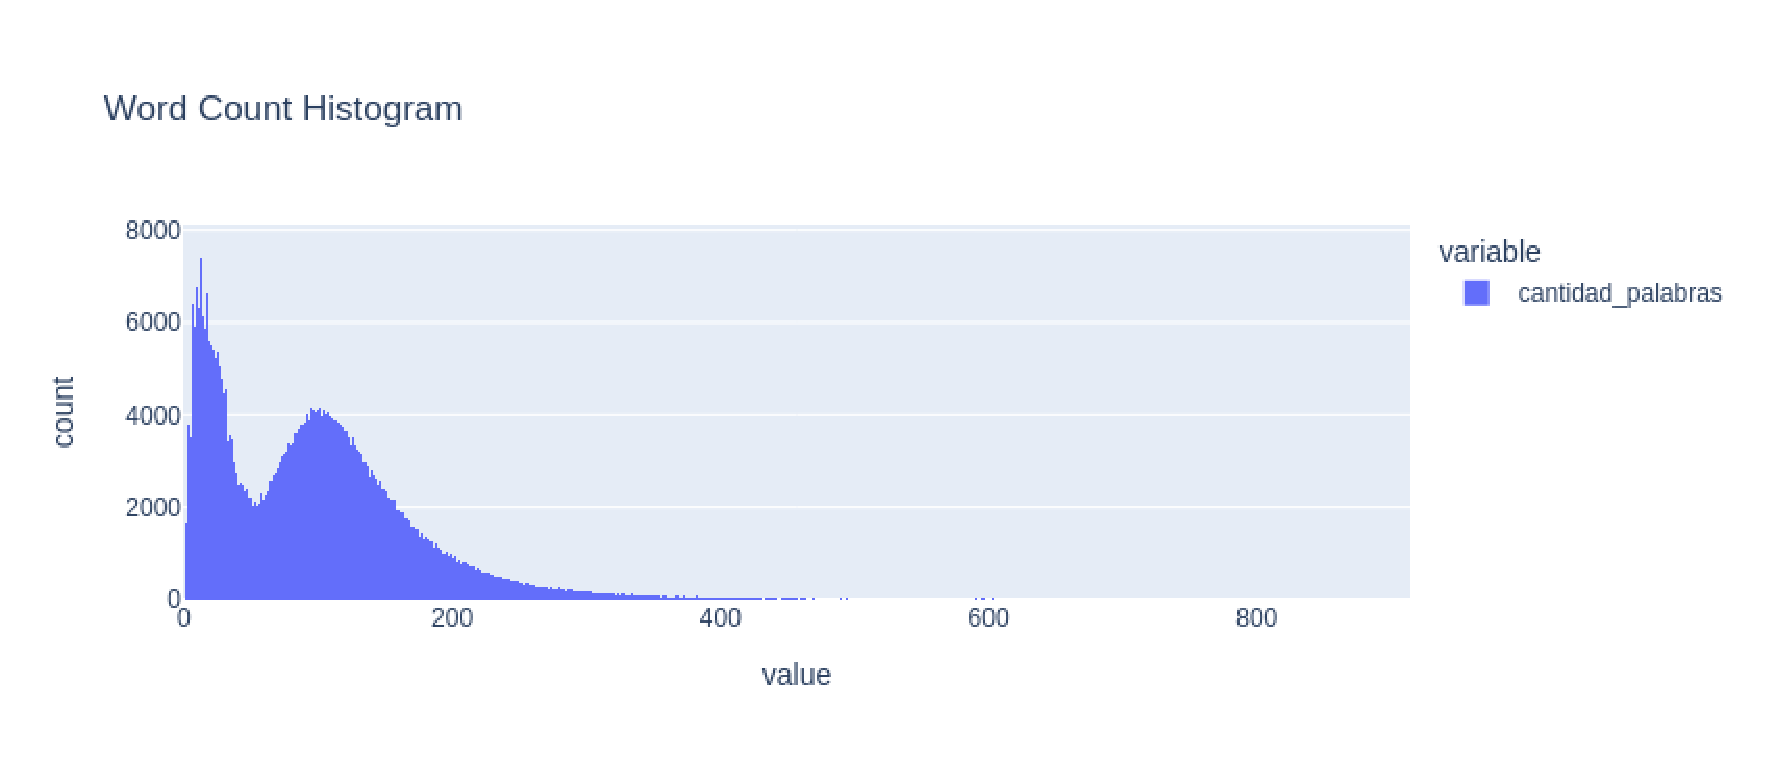
\includegraphics[width=\textwidth]{imgs/histograma.eps}
%     \caption{Histogram of Word Count $l_w$ in Corpus $D^T$}
%     \label{fig:histogramalw}
% \end{figure}
% \begin{figure}[!t]
%     \centering
%     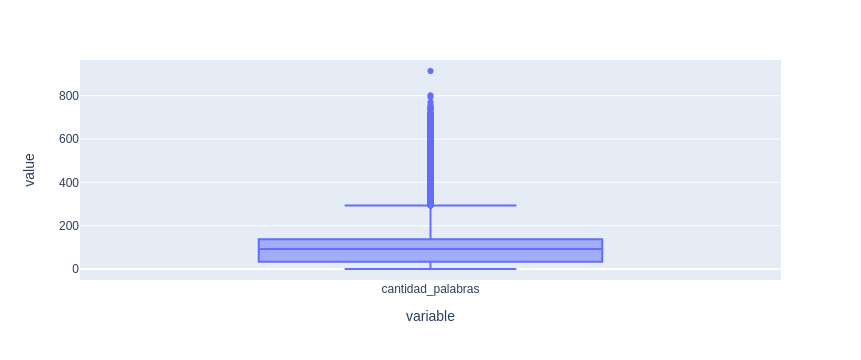
\includegraphics[width=\textwidth]{imgs/boxplot.png}
%     \caption{Box Plot of Word Count $l_w$ in Corpus $D^T$}
%     \label{fig:boxplotlw}
% \end{figure}

% \begin{figure}[!t]
%     \centering
%     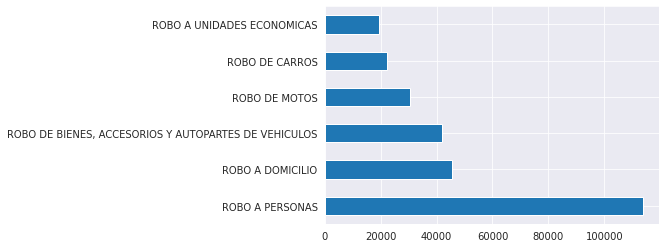
\includegraphics[width=\textwidth]{imgs/categorias.png}
%     \caption{Text Categories of Dataset $D^T$}
%     \label{fig:categorias}
% \end{figure}

% \begin{table}[!t]
% \caption{Statistical Values of the Dataset}
% \label{tab: metricasorig}
% \centering
% \begin{tabular}{c c}
% \hline
% \textbf{Metric} & \textbf{Value} \\
% \hline
% Count &    \numprint{671146} \\ %count
% Mean     &   \numprint{98.34} \\ %mean
% Std      &   \numprint{77.38} \\ %std
% Min      &    \numprint{0} \\ %min
% 25\%      &   \numprint{33.00} \\
% 50\%      &   \numprint{92.00} \\
% 75\%      &  \numprint{137.00} \\
% Max      &  \numprint{914.00} \\
% \hline
% \end{tabular}
% \end{table}
% ==================== figures and tables ====================
The dataset \( D^T_{\kappa=6, N} \) was partitioned into training
(\( D^T_{\kappa=6,train} \)), validation (\( D^T_{\kappa=6, valid} \)), and testing
(\( D^T_{\kappa=6, test} \)) subsets to facilitate model training and
evaluation. The training set comprises 273,336 records (63.32\% of the
dataset), while the validation and test sets contain 68,333 (15.83\%)
and 90,000 (20.85\%) records, respectively. The validation set was
derived by splitting the training data in an 80:20 ratio. %Table
% \ref{tab:datasplit} summarizes the distribution of records across
% these subsets, ensuring a balanced allocation for model development
% and assessment.

\subsubsection{Extended Taxonomy (\(D_{\kappa=11}\)) Dataset}
\label{sec:extended-dataset}
We constructed an extended target dataset comprising 11 distinct
categories by integrating police reports with corresponding
prosecutor's office records. This integration significantly expanded
our training corpus, enhancing the model's exposure to diverse textual
patterns. The final dataset contains \numprint{1109335} records, with
the distribution across categories detailed in
Table~\ref{tab:GeneracionDataset}. The dataset creation process
involved the following steps:

\begin{enumerate}
\item \textbf{Initial Data Extraction:}Crime reports from 2014–2022 were extracted and filtered for
  robbery cases from \printInicialesComision, yielding to
  \numprint{735045} records.
  \item \textbf{Narrative Retrieval:} Crime narratives are obtained
    for each of the previous records obtaining a total of
    \numprint{725079}. However, non-robbery cases are excluded if
    found. This produces a total of \numprint{723435} records.
  \item \textbf{Preprocessing:} lowercasing and removal of
    non-alphanumeric characters.
  \item \textbf{Dataset Integration:}Police and prosecutor narratives
    were combined into a single dataset, yielding to
    \numprint{1446870} records.
  \item \textbf{Quality Control:} statistical analysis over the text
    is carried out. Narratives with 50–400 words were retained (upper
    fence: 389.5 words), reducing the dataset to \numprint{1140728}
    records. Crime labels were also standardized (e.g. removing accents).
  \item \textbf{Category refinement:} Non-compliant labels (48
    categories) were discarded with the exception of the
    \textit{OTHER ROBBERIES} category which is retained. The final dataset, with
    \numprint{1109335} records was randomly shuffled and
  \item \textbf{Dataset Split:} The dataset is partition into training
    (\numprint{807468} samples $\approx$ 72\%), validation
    (\numprint{201867} samples  $\approx$ 18\%),  and test
    (\numprint{100000} samples $\approx$ 10\%) sets.
\end{enumerate}

\begin{table}[htbp]
    \centering
    \caption{Extended Taxonomy Dataset}
    \label{tab:GeneracionDataset}
    \scriptsize
    \begin{tabularx}{\textwidth}{p{0.4\textwidth}p{0.4\textwidth}X}
        \toprule
        Basic Taxonomy & Extended Labels & Total \\ \hline
        HOME ROBBERY & HOME ROBBERY & \numprint{172264} \\
        STREET ROBBERY & STREET ROBBERY & \numprint{421497} \\ 
        BUSINESS ROBBERY & BUSINESS ROBBERY & \numprint{74088} \\ 
        VEHICLE PARTS AND ACCESSORIES THEFT & VEHICLE PARTS AND ACCESSORIES THEFT & \numprint{154546} \\
        CAR THEFT & CAR THEFT & \numprint{90038} \\ 
        MOTORCYCLE THEFT & MOTORCYCLE THEFT & \numprint{119128} \\ \hline 
        \multirow{4}{*}{NO INFORMATION}  & OTHER ROBBERIES & \numprint{43468} \\ 
        {} & WATER VESSEL ROBBERY & \numprint{9407} \\ 
        {} & SOCIAL ORGANIZATION ROBBERY & \numprint{3087} \\ 
        {} & EDUCATIONAL INSTITUTION ROBBERY & \numprint{17252} \\
        {} & PUBLIC INSTITUTION ROBBERY & \numprint{4560} \\ \hline
        \multicolumn{2}{c}{Total} & \numprint{1109335} \\
        \bottomrule
    \end{tabularx}
  \end{table}

\subsection{Model Training}
\label{sec:model-training}

  
% \section{First Section}
% \subsection{A Subsection Sample}
% Please note that the first paragraph of a section or subsection is
% not indented. The first paragraph that follows a table, figure,
% equation etc. does not need an indent, either.

% Subsequent paragraphs, however, are indented.

% \subsubsection{Sample Heading (Third Level)} Only two levels of
% headings should be numbered. Lower level headings remain unnumbered;
% they are formatted as run-in headings.

% \paragraph{Sample Heading (Fourth Level)}
% The contribution should contain no more than four levels of
% headings. Table~\ref{tab1} gives a summary of all heading levels.

% \begin{table}
% \caption{Table captions should be placed above the
% tables.}\label{tab1}
% \begin{tabular}{|l|l|l|}
% \hline
% Heading level &  Example & Font size and style\\
% \hline
% Title (centered) &  {\Large\bfseries Lecture Notes} & 14 point, bold\\
% 1st-level heading &  {\large\bfseries 1 Introduction} & 12 point, bold\\
% 2nd-level heading & {\bfseries 2.1 Printing Area} & 10 point, bold\\
% 3rd-level heading & {\bfseries Run-in Heading in Bold.} Text follows & 10 point, bold\\
% 4th-level heading & {\itshape Lowest Level Heading.} Text follows & 10 point, italic\\
% \hline
% \end{tabular}
% \end{table}


% \noindent Displayed equations are centered and set on a separate
% line.
% \begin{equation}
% x + y = z
% \end{equation}
% Please try to avoid rasterized images for line-art diagrams and
% schemas. Whenever possible, use vector graphics instead (see
% Fig.~\ref{fig1}).

% \begin{figure}
% \includegraphics[width=\textwidth]{./fig1.eps}
% \caption{A figure caption is always placed below the illustration.
% Please note that short captions are centered, while long ones are
% justified by the macro package automatically.} \label{fig1}
% \end{figure}

% \begin{theorem}
% This is a sample theorem. The run-in heading is set in bold, while
% the following text appears in italics. Definitions, lemmas,
% propositions, and corollaries are styled the same way.
% \end{theorem}
% %
% % the environments 'definition', 'lemma', 'proposition', 'corollary',
% % 'remark', and 'example' are defined in the LLNCS documentclass as well.
% %
% \begin{proof}
% Proofs, examples, and remarks have the initial word in italics,
% while the following text appears in normal font.
% \end{proof}
% For citations of references, we prefer the use of square brackets
% and consecutive numbers. Citations using labels or the author/year
% convention are also acceptable. The following bibliography provides
% a sample reference list with entries for journal
% articles~\cite{ref_article1}, an LNCS chapter~\cite{ref_lncs1}, a
% book~\cite{ref_book1}, proceedings without editors~\cite{ref_proc1},
% and a homepage~\cite{ref_url1}. Multiple citations are grouped
% \cite{ref_article1,ref_lncs1,ref_book1},
% \cite{ref_article1,ref_book1,ref_proc1,ref_url1}.

% \begin{credits}
% \subsubsection{\ackname} A bold run-in heading in small font size at the end of the paper is
% used for general acknowledgments, for example: This study was funded
% by X (grant number Y).

% \subsubsection{\discintname}
% It is now necessary to declare any competing interests or to specifically
% state that the authors have no competing interests. Please place the
% statement with a bold run-in heading in small font size beneath the
% (optional) acknowledgments\footnote{If EquinOCS, our proceedings submission
% system, is used, then the disclaimer can be provided directly in the system.},
% for example: The authors have no competing interests to declare that are
% relevant to the content of this article. Or: Author A has received research
% grants from Company W. Author B has received a speaker honorarium from
% Company X and owns stock in Company Y. Author C is a member of committee Z.
% \end{credits}
% %
% ---- Bibliography ----
%
% BibTeX users should specify bibliography style 'splncs04'.
% References will then be sorted and formatted in the correct style.
%
\bibliographystyle{splncs04}
\bibliography{bibliography}
%
% \begin{thebibliography}{8}
% \bibitem{ref_article1}
% Author, F.: Article title. Journal \textbf{2}(5), 99--110 (2016)

% \bibitem{ref_lncs1}
% Author, F., Author, S.: Title of a proceedings paper. In: Editor,
% F., Editor, S. (eds.) CONFERENCE 2016, LNCS, vol. 9999, pp. 1--13.
% Springer, Heidelberg (2016). \doi{10.10007/1234567890}

% \bibitem{ref_book1}
% Author, F., Author, S., Author, T.: Book title. 2nd edn. Publisher,
% Location (1999)

% \bibitem{ref_proc1}
% Author, A.-B.: Contribution title. In: 9th International Proceedings
% on Proceedings, pp. 1--2. Publisher, Location (2010)

% \bibitem{ref_url1}
% LNCS Homepage, \url{http://www.springer.com/lncs}, last accessed 2023/10/25
% \end{thebibliography}
\end{document}

%%% Local Variables:
%%% mode: LaTeX
%%% TeX-master: t
%%% End:
